\documentclass[14pt, titlepage,fleqn]{extarticle}
\usepackage[T1,T2A]{fontenc}
\usepackage[utf8]{inputenc}

\usepackage{amsmath}
\usepackage[russian]{babel}

\usepackage{titlepage}
\usepackage[final]{pdfpages}
\usepackage{listings}
\usepackage{color}
\usepackage{graphicx}
\usepackage{float} 

\usepackage{caption}


\newcommand{\InsertGraf}[2]{
	\begin{figure}[H]
		\center{\includegraphics[width = 1\textwidth]{#1}}
		\caption{#2}
	\end{figure}
}

\definecolor{dkgreen}{rgb}{0,0.6,0}
\definecolor{gray}{rgb}{0.5,0.5,0.5}
\definecolor{mauve}{rgb}{0.58,0,0.82}


\lstset{frame=single,
	language=Python,
	aboveskip=3mm,
	belowskip=3mm,
	showstringspaces=false,
	columns=flexible,
	basicstyle={\small\ttfamily},
	numbers=none,
	numberstyle=\tiny\color{gray},
	keywordstyle=\color{blue},
	commentstyle=\color{dkgreen},
	stringstyle=\color{mauve},
	breaklines=true,
	breakatwhitespace=true,
	tabsize=3
}

\begin{document}
	\selectlanguage{russian}
	

	\fefutitlepage{Б9119-02.03.01сцт}{Панченко Н.К.}{17}{мая}{22}
	
	
	\newpage
	
 
	\clearpage
	\section*{Постановка задачи}
	Дана матричная игра с матрицей $A$ размерности 6х8. Необходимо вычислить верхнюю и нижнюю цены игры, а также найти равновесное решение в смешанных стратегиях.
	\section*{Реализация нахождения верхней и нижней цен игры}
	Для реализации воспользуемся языком программирования Python.
	\begin{lstlisting}
		def findTopPrice (A, n, m):
		maxs = [ ]
		for i in range(m):
			max = A[0, i]
			for j in range(1, n):
				if (A[j, i] > max):
					max = A[j, i]
					maxs.append (max )
		return min ( maxs )
	
	def findBottomPrice(A, n , m):
		mins = [ ]
		for i in range(n):
			min = A[i, 0]
			for j in range(1, m):
				if (A[i, j] < min):
					min = A[i, j]
					mins.append(min)
		return max (mins)	
	\end{lstlisting}
	\section*{Реализация алгоритма для нахождения решения}
	Для реализации воспользуемся языком программирования Python и библиотекой Numpy для удобной работы с матрицами.
	\begin{lstlisting}
import numpy as np
import copy

n = 6
m = 8

A = np.random.randint(1, 10, (m, n)).astype('float')
b = np.random.randint(1, 10, m).astype('float')
c = np.random.randint(1, 10, n).astype('float')

startC = copy.deepcopy(c)
startB = copy.deepcopy(b)
prevLeads = []
c = c*(-1)
cFree = 0

colInd = [i for i in range(0, n)]
prevLeads.append(copy.deepcopy(colInd))
strInd = [i for i in range(n, n+m)]


while min(c) < 0:
oldColInd = copy.deepcopy(colInd)
    oldStrInd = copy.deepcopy(strInd)

    changeC = copy.deepcopy(c)
    check = True

    while check:
        check = False

        leadCol = np.argmax(np.abs(changeC))
        leadStr = 0
        leadStrVal = 100000000000000000

        for i in range(0, m):
            if (not((b[i] > 0) and (A[i, leadCol] < 0))):
                leadStrNew = b[i] / A[i, leadCol]
                if (leadStrNew < leadStrVal):
                    leadStr = i
                    leadStrVal = leadStrNew


        leadVal = copy.deepcopy(A[leadStr, leadCol])


        strInd = np.insert(strInd, 0, colInd[leadCol])
        colInd[leadCol] = copy.deepcopy(strInd[leadStr+1])
        strInd = np.delete(strInd, leadStr + 1)


        for i in range(len(prevLeads)):
            prevLeads[i].sort()
            sortColInd = copy.deepcopy(colInd)
            sortColInd.sort()
            if prevLeads[i] == sortColInd:
                changeC[leadCol] = 0
                colInd = copy.deepcopy(oldColInd)
                strInd = copy.deepcopy(oldStrInd)
                check = True
                break

    prevLeads.append(copy.deepcopy(colInd))


    helpVals = copy.deepcopy(A[:, leadCol]*(-1))
    helpVals = np.delete(helpVals, leadStr)


    leadStrVals = A[leadStr]
    leadB = b[leadStr]

    A = np.delete(A, leadStr, 0)
    b = np.delete(b, leadStr)
    A = np.reshape(np.insert(A, 0, [0 for i in range(0, n)]), (m, n))
    b = np.insert(b, 0, 0)

    for i in range(0, n):
        if i != leadCol:
            A[0, i] = leadStrVals[i]/leadVal
    A[0, leadCol] = 1/leadVal

    b[0] = leadB/leadVal


    for i in range(1, m):
        for j in range(0, n):
            oldVal = A[i, j]
            A[i, j] = A[0, j]*helpVals[i-1]
            if (oldColInd[j] == colInd[j]):
                A[i, j] += oldVal
        b[i] = b[0]*helpVals[i-1] + b[i]


    leadC = c[leadCol]


    for i in range(0, n):
        oldVal = c[i]
        c[i] = A[0, i] * leadC *(-1)
        if (oldColInd[i] == colInd[i]):
            c[i] += oldVal
    cFree = b[0] * leadC*(-1) + cFree

print()

res = 0
for i in range(0, n):
    if i in strInd:
        print("x_" + str(i) + " = " + str(b[list(strInd).index(i)]) + " ", end='')
    else:
        print("x_" + str(i) + " = " + str(0) + " ", end='')

print()
check = False
for i in range(0, n):
    if i in strInd:
        if check:
            print(" + ", end='')
        print(str(startC[i]) +" * " + str(b[list(strInd).index(i)]), end='')
        res += startC[i]*b[list(strInd).index(i)]
        check = True


print(" = " + str(res))

res = 0

for i in range(n, n+m):
    if i in colInd:
        print("y_" + str(i-n) + " = " + str(c[list(colInd).index(i)]) + " ", end='')
    else:
        print("y_" + str(i-n) + " = " + str(0) + " ", end='')

check = False
for i in range(n, n+m):
    if i in colInd:
        if check:
            print(" + ", end='')
        print(str(startB[i-n]) +" * " + str(c[list(colInd).index(i)]), end='')
        res += startB[i-n]*c[list(colInd).index(i)]
        check = True

print(" = " + str(res))
\end{lstlisting}

	\section*{Тесты}
        \begin{figure}[H]
            \center{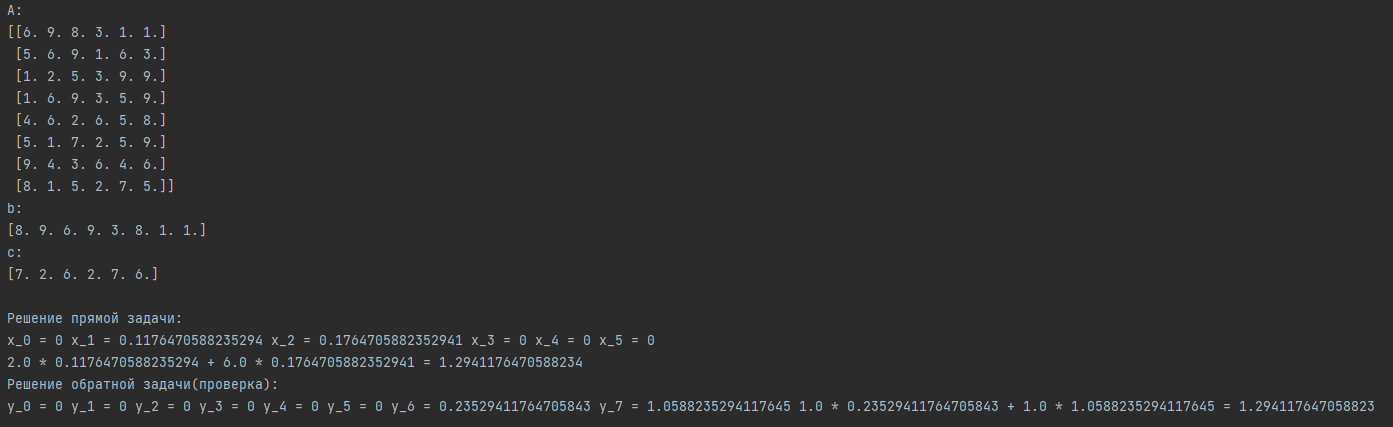
\includegraphics[width = 1\textwidth]{Картинки/lb4.png}}
        \end{figure}

    


	\newpage
	\section*{Заключение}
	В ходе данной лабораторной работы был реализован алгоритм нахождения верхней и нижней цен игры, а также разработана программа, позволяющая находить решения прямой и двойственных задач линейной оптимизации симплекс-методом.
\end{document}